\chapter{Implementation}

\section{Preprocessing}
\begin{itemize}
    \item data from \cref{sec:data-ana} is used for preprocessing
    \item Load data from the CSV files.
    \item Concatenate data from the first 10 lines of each file.
    \item Replace missing \acs{bssid} value
    \item Create a target variable.
    \item Normalize the data.
    \item Create sequences of data based on window_size.
    \item Encode the target variable.
    \item Split the data into training and testing sets.
\end{itemize}

\begin{figure}
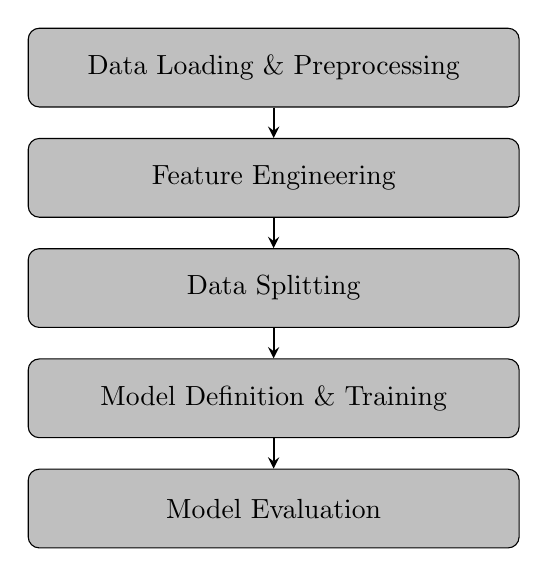
\begin{tikzpicture}[scale=0.7]
    % Define the styles for the processes and arrows
    \tikzstyle{process}=[rectangle, rounded corners, draw=black, fill=lightgray, text centered, text width=6cm, minimum height=1cm]
    \tikzstyle{arrow}=[thick,->,>=stealth]

    % Draw the processes
    \node[process] (data_loading) at (0, 0) {Data Loading \& Preprocessing};
    \node[process] (feature_engineering) at (0, -2) {Feature Engineering};
    \node[process] (data_splitting) at (0, -4) {Data Splitting};
    \node[process] (model_definition) at (0, -6) {Model Definition \& Training};
    \node[process] (model_evaluation) at (0, -8) {Model Evaluation};

    % Draw the arrows between the processes
    \draw[arrow] (data_loading) -- (feature_engineering);
    \draw[arrow] (feature_engineering) -- (data_splitting);
    \draw[arrow] (data_splitting) -- (model_definition);
    \draw[arrow] (model_definition) -- (model_evaluation);
\end{tikzpicture}

\caption{Flow diagram of the LSTM implementation process.}
\label{fig:flow_diagram}
\end{figure} 


\section{\ac{lstm}}
\begin{itemize}
    \item Decision in previous chapter for \ac{lstm}
    \item LSTM layer with 1000 units.
    \item Dense layer with softmax activation (number of units equal to the number of categories in the target variable).
\end{itemize}

\section{Training}

\begin{figure}
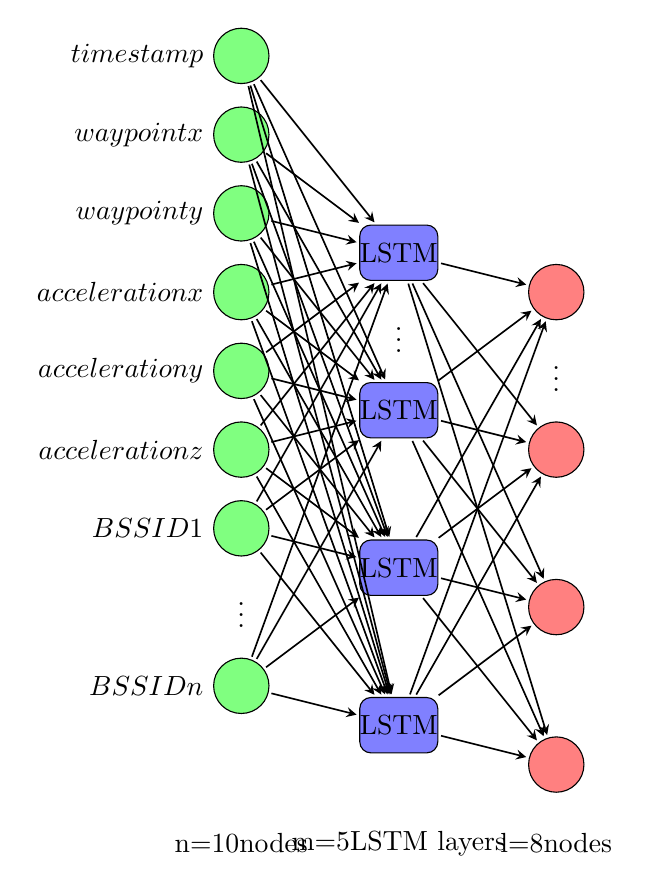
\begin{tikzpicture}[
     % Define styles
     input neuron/.style={draw, fill=green!50, circle, minimum size=20pt, inner sep=0pt},
     lstm neuron/.style={draw, fill=blue!50, rectangle, rounded corners, minimum size=20pt, inner sep=0pt},
     output neuron/.style={draw, fill=red!50, circle, minimum size=20pt, inner sep=0pt},
     arrow/.style={->, >=stealth, shorten >=1pt, shorten <=1pt, semithick}
 ]
 
 % Parameters for number of nodes
 \def\n{10}
 \def\m{5}
 \def\l{8}
 
 % Input layer
 \foreach \name/\y/\label in {1/7/$\text{timestamp}$, 2/6/$\text{waypoint x}$, 3/5/$\text{waypoint y}$, 4/4/$\text{acceleration x}$, 5/3/$\text{acceleration y}$, 6/2/$\text{acceleration z}$, 7/1/$\text{BSSID 1}$, 8/-1/$\text{BSSID n}$}
     \node[input neuron, label=left:\label] (I-\name) at (0,\y) {};
 \node at (0,-3) {n=\n nodes};
 
 % Dots for input layer
 \node at (0,0) {$\vdots$};
 
 % LSTM layers
 \foreach \y [count=\name] in {4.5,2.5,0.5,-1.5}
     \node[lstm neuron] (L-\name) at (2,\y) {LSTM};
 \node at (2,-3) {m=\m LSTM layers};
 
 % Dots for LSTM layer
 \node at (2,3.5) {$\vdots$};
 
 % Output layer
 \foreach \name/\y in {1/4, 2/2, 3/0, 4/-2}
     \node[output neuron] (O-\name) at (4,\y) {};
 \node at (4,-3) {l=\l nodes};
 
 % Dots for output layer
 \node at (4,3) {$\vdots$};
 
 % Connect input layer to LSTM
 \foreach \i in {1,...,8}
     \foreach \j in {1,...,4}
         \draw[arrow] (I-\i) -- (L-\j);
 
 % Connect LSTM to output layer
 \foreach \i in {1,...,4}
     \foreach \j in {1,...,4}
         \draw[arrow] (L-\i) -- (O-\j);

\end{tikzpicture}
\caption{LSTM neural network architecture.}
\label{fig:lstm_architecture}
\end{figure}
    
    
%\noindent
